\documentclass[11pt]{article}


\usepackage{amssymb}
\usepackage[applemac]{inputenc} 
\usepackage{epsfig}
\usepackage{graphicx} 
%\usepackage{psfrag}
\usepackage{amsmath}
\usepackage{amsfonts}
%\usepackage[francais]{babel}
%\usepackage{fancyhdr}
\usepackage{color}
\usepackage{pdfpages}

\textwidth14.5cm
\textheight21.0cm
\oddsidemargin0.9cm
\topmargin-0.8cm
\newlength{\plarg}
\setlength{\plarg}{14cm}
\newlength{\glarg}
\setlength{\glarg}{17cm}

\newcommand{\beq}{\begin{equation}}
\newcommand{\eeq}{\end{equation}}


\begin{document}
\title{Report of the AMMM Projet}
\author{{\Large \bf Mathieu Chiavassa, Anthony Nixon}\\
{\it Master MIRI Data Science,  FIB, BarcelonaTech, UPC}}

\maketitle


\tableofcontents
\pagebreak`
%%%%%%%%%%%%%%%%%%%
%\part{Problem statement}
\section{Problem statement}
\label{sec-pbsetting}
The problem we have to solve is to find an optimal daily schedule for a given number of nurses in an hospital. The optimal workload is given by the hospital for all the hours of the day. 
The nurses schedule must satisfiy a list of constraints. \\
To model the problem, we introduce the following input parameters : 
\begin{itemize}
\item $numNurses$ : Number of nurses available 
\item $hours$ : Total number of hours in one working day
\item $demand$ : Vector representing the number of nurses who are supposed to work at each hours
\item $minHours$ : Minimal number of working hours for a given nurse
\item $maxHours$ : Maximal number of working hours for a given nurse
\item $maxConsec$ : Maximal allowed number of consecutive working hours  for a given nurse
\item $maxPresence$ : Maximal number of hours the nurses can spend at the hospital for a given nurse
\end{itemize}

\noindent
With these parameters, we  can introduce the different constraints :
\begin{itemize}
\item[C1 :] For each hour $h$, at least, $demand[h]$ nurses should be working
\item[C2 :] Each nurse should work at least $minHours$ hours 
\item[C3 :] Each nurse should work at most $maxHours$ hours 
\item[C4 :] Each nurse should work at most $maxConsec$ consecutive hours
\item[C5 :] No nurse can stay at the hospital for more than $maxPresence$ hours
\item[C6 :] No nurse can rest for more than one consecutive hour
\end{itemize}

The project consists in solving this problem using three different optimization methods: the linear model with the OPL software and the two metaheuristic methods  BRKGA and GRASP.

\pagebreak

\section{Linear model for optimization in OPL}
\label{sec-OPL}
In order to solve this optimization problem in OPL we used the aforementioned parameters but we also introduce the following ones : 
\begin{itemize}
\item range N : Range between 1 and $numNurses$
\item range H : Range between 1 and $hours$
\item works[numNurses][hours] : Boolean matrix of size $numNurses*hours$. \\
Tells for each nurse if he/she is working at a given hour,i.e, if $works[i][j]=1$ then the nurse $i$ is working during the hour $j$
\item worksBefore[numNurses][hours] : Boolean matrix of size $numNurses*hours$
\item worksAfter[numNurses][hours] : Boolean matrix of size $numNurses*hours$
\item rests[numNurses][hours] : Boolean matrix of size $numNurses*hours$
\item used[numNurses] : Boolean vector telling if a nurse is working during the day (value 1) or not (value 0). \\
\end{itemize}
\vskip.1cm
\noindent
The objective function to be minimized is therefore $$\sum_{i=1}^{n} used[i].$$
The solution must satisfy the aforementioned constraints C1 to C6 we expressed in the following form to be used by the OPL code:
\begin{itemize}
\item[C1 :] $\forall h$,  $\displaystyle{\sum_{i=1}^{n} }works[i][h] \geq demand[h]$ \\
For each hour, the sum of nurses working should be greater or equal than the number of nurses needed.    
\item[C2 :] $\forall n$,  $\displaystyle{\sum_{i=1}^{h}} works[n][i] \geq minHours*used[n]$\\
For each nurse, the sum of working hours in her schedule should be greater or equal than the minimum number of working hours.
\item[C3 :] $\forall n$,  $\displaystyle{\sum_{i=1}^{h}} works[n][i] \leq maxHours*used[n]$ \\
For each nurse, the sum of working hours in her schedule should be lower or equal than the maximum number of working hours.
\item[C4 :] $\forall n$, $\forall j\in[1; hours-maxConsec]$, $\displaystyle{\sum_{i=j}^{j+maxConsec}} works[n][i] \leq maxConsec*used[n]$ 
\item[C5 :] $\forall n$, $\forall h$ if $h \leq hours-maxPresence$ :\\$worksBefore[n][h]+worksAfter[n][h+maxPresence] \leq 1$
\item[C6 :] $\forall n$, $\forall h\leq hours-1$ : \\$worksAfter[n][h] \geq worksAfter[n][h+1]$\\$worksBefore[n][h] \leq worksBefore[n][h+1]$\\$rests[n][h]+rests[n][h+1]\leq 1$\\$rests[n][h] = (1-works[n][h]) - (1-worksAfter[n][h]) - (1-worksBefore[n][h])$ \\
\end{itemize}

\noindent
The full  OPL code in written the appendix \ref{appenOPL}.

\subsection{Results for the OPL code}
In this section, we are going to present 3 tests based on 3 different datasets, a small one (TEST1), a medium one (TEST2), and a big one (TEST3). The different datasets are in the OPL data file. \\

\noindent
{\bf TEST1}:\\
In this test we try to optimize the schedule of 30 nurses for a 9 hours working day, with the following demand workload : \\
{\tt demand = [ 5 3 8 5 1 7 5 6 2 ];}\\
And the following nurses parameters:\\
{\tt numNurses = 30;
 hours =  9;
 minHours = 3;
 maxHours = 6;
 maxConsec = 7;
 maxPresence = 8;}\\

On this small dataset, OPL took less than 1 second to find the optimal solution. The objective function is equal to $8$, which is the max of the demand vector. It means that not a single nurse is useless, and the solution is optimal. \\

\noindent
{\bf TEST2}:\\
In this test we try to optimize the schedule of 200 nurses for a 24 hours working day, with the following demand workload : \\
{\tt demand = [ 53 24 33 40 70 12 33 55 66 12 30 22 55 77 88 22 34 55 22 55 23 22 11 12 ];}\\
And the following nurses parameters:\\
{\tt numNurses = 200;
 hours =  24;
 minHours = 6;
 maxHours = 12;
 maxConsec = 6;
 maxPresence = 18;}\\

OPL took only 3 minutes to solve this problem. But the objective function value is $108$, which is higher than the max of the demand vector, so we are not sure if we can assume that this is the optimal solution. \\

\noindent
{\bf TEST3}:\\
In this test we try to optimize the schedule of 1800 nurses for a 24 hours working day, with the following demand workload : \\
{\tt demand = [964 650 966 1021 824 387 828 952 611 468 403 561 862 597 1098 855 918 1016 897 356 615 670 826 349]; }\\
And the following nurses parameters:\\
{\tt numNurses = 1800;
 hours =  24;
 minHours = 6;
 maxHours = 18;
 maxConsec = 7;
 maxPresence = 24;}\\

Since it is a very huge dataset, OPL took 1 hour and 13 minutes to optimize this problem. But the result is excellent, the objective function is equal to $1098$ nurses, which is the max of the demand vector. So we can be sure that this solution is the optimal solution. 

\pagebreak

%%%%%%%%%%%%%%. BRKGA  PART %%%%%%%%%%%
\section{The BRKGA method}
In this section, we use a Biased Random Key Genetic Algorithm (BRKGA), to solve the nurses scheduling problem. This method belongs to the genetic algorithms family and has been introduced by Bean (1994) and developed later for solving large combinatorial optimization problems. The basic principle is to mimic the evolution of individuals in a population submitted to natural selection. Basically, for a given criteria, called {\it fitness}, the best individuals are selected and are crossed with the other individuals of the population. Generations after generations, the individuals that optimize the fitness are selected.\\
We based our work in this section on the paper of Jos\'e Fernando Goncalves and Mauricio G. C. Resende, {\it  Biased Random-Key Genetic Algorithm for Combinatorial Optimization} and on the python code provided by profesor M. Ruiz Ramirez.\\

Each individual of the population is represented by a {\it chromosome} and corresponds to a candidate for the solution we are looking for.
 The chromosome consists of a given number of {\it genes} that takes a real value in the interval $[0,1]$. The gene are  used to compute the fitness of the individual which is correlated to the problem we want to optimize.
To solve a minimization problem such the nurse scheduling described in section \ref{sec-pbsetting}, the BRKGA used the following steps:
\begin{itemize}
\item[1] define the size $p$ of the population, and the number of generations
\item[2] initialize randomly the genes of the $p$ individuals
\item[3] decode the genes to compute the fitness of each individual
\item[4] select the best individuals, {\it elite}, and generate the next generation chromosomes, see figure \ref{fig-brkga}
\item[5] go to step 3 until the number of generations is not reached
\item[6] decode the best fitness chromosome of the last generation 
\end{itemize}
If the problem and the parameters have been chosen correctly, the individual with the best fitness in the last generation is a good candidate for the optimum of our problem.\\

\begin{figure}[htbp]
\begin{center}
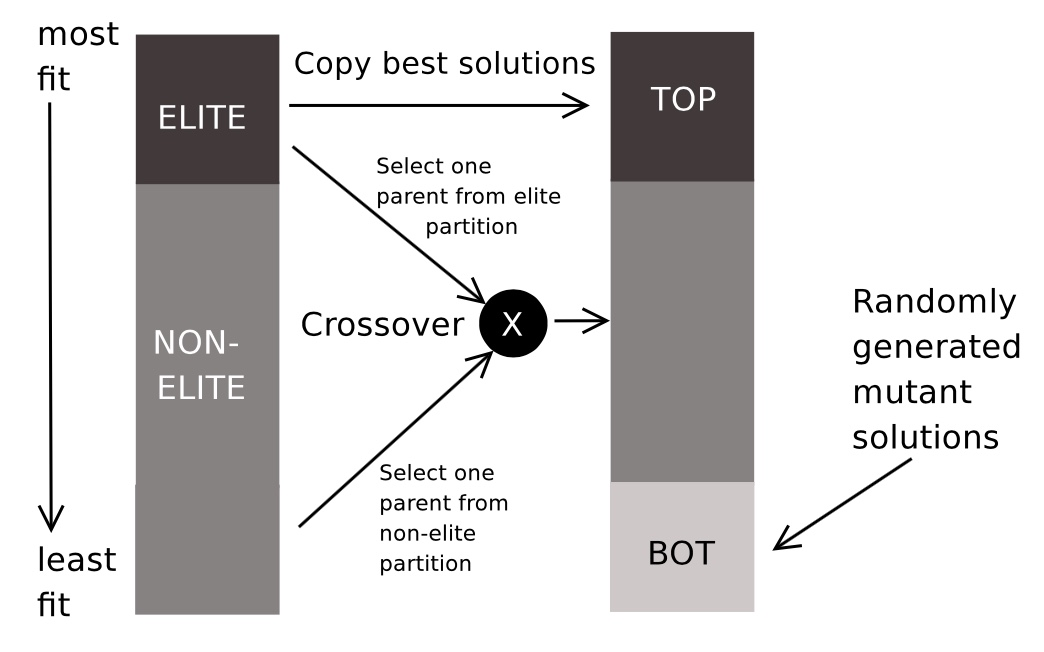
\includegraphics[scale=0.38]{./figBRKGA} 
\end{center}
\caption{Schematic representation for transition to generation $k$ to $k+1$. (Reproduced from J.F. Goncalves paper). A percentage of the best fitted individuals, called elite is directly reproduced in the next generation. A percentage of the new generation is composed by crossover between elite and non-elite individuals. Crossover is obtain by randomly exchanging genes of the parents. The third part of the new generation is composed by mutants whose genes are randomly generated. This allows to explore a larger space of solutions, and prevents (theoretically) to be trapped in a local optimum. }
\label{fig-brkga}
\end{figure}

The tricky part of the BRKGA algorithms is the decoder procedure and a huge number of research papers deal with this problem.
 If the chromosome is composed of N genes, the decoder must map the hypercube space $[0,1]^N$ to the solution space. A suited fitness has also to be defined o select the best candidate in the solution space. \\
 
We read many papers to find the best way to define such procedure for our nurse scheduling problem. Nevertheless we do not succeed to apply the proposed ideas due to the constraints we have on the schedules. We then proposed our own decoder technique, which as we will see, works well in some cases but has some weakness we will comment later on.\\

\subsection{Our decoder and fitness procedures}
The decoder procedure we propose  will map the chromosome  to the daily schedule for all the nurses, represented by the boolean array $works$ of size $numNnurse \times hours$ introduced in section \ref{sec-OPL}. The chromosome length is therefore $numNurse \times hours$. The mapping from floating genes value to boolean ones is simply done by the transform procedure:\\

\noindent
{\tt {\bf Procedure transform}\\
for all the genes of the population\\
\hspace*{.2cm} if gene\_value $\leq$ 1-minHours/hours then solution\_value$=$0\\
 \hspace*{.2cm} else solution\_value$=$1\\
}
\vskip.2cm
\noindent
With this procedure, the probability of working for a nurse depends on the percentage she has to work during the day. If the ratio is small, then the transform procedure will produce more 0 values (not work). On the contrary  more values 1 will be produced. (This improves significantly the results in our experiments comparing to use  the fixed value 0.5).\\
 
 \vskip.2cm
\noindent
Once we have the daily schedule, we will check if the schedule satisfies all the constraints of the problem described in section \ref{sec-pbsetting} and define a corresponding value of the fitness. First for a given nurse, its schedule is verified:\\

\noindent
{\tt {\bf Procedure checkschedule}\\
test=0\\
\hspace*{.2cm} check all the constraints from C2 to C6 defined in section \ref{sec-pbsetting}\\
\hspace*{.2cm} for each non satisfied constraint do test $+=$ 1\\
return test\\
}
\vskip.2cm
\noindent
The way we check in practice the constraints is detailled in the procedure {\tt checkschedule} in Annexe \ref{appendBRKGA}. The value of test will be used for the fitness.\\

\noindent
We then compare the workload of the day with the theoretical demand specified by the user, in order to check if the constraint C1 is satisfied:\\

\noindent
{\tt {\bf Procedure compareworkload}\\
error=0\\
for all the hours $h$ of the day\\
\hspace*{.2cm}compute the number of working nurses: workload(h)\\
\hspace*{.2cm}if workload(h) $>$ demand(h) then error $+=$ workload(h)-demand(h)\\
\hspace*{.2cm}if workload(h) $<$ demand(h) then error $+=$ 10*$|$workload(h)-demand(h)$|$\\
return error\\
}
\vskip.2cm
\noindent
For this error we penalize 10 times more the fact that the workload is less than the demand. When the error is larger than the demand, the optimal soltuion is not reached, but the solution is acceptable in practice. If the workload is exactly aquals to the demand, the error is 0. \\

\noindent
We can then define the complete decode procedure \\

\noindent
{\tt {\bf Procedure decode}\\
 transform\\
for all the individuals in the population\\
\hspace*{.2cm} fitness=0\\
\hspace*{.2cm} for all the nurses\\
\hspace*{.6cm} test=checkschedule\\
\hspace*{.6cm} fitness $+=$ 10.*test/numNurses\\
\hspace*{.2cm} error=compareworkload\\
\hspace*{.2cm} fitness $+=$ error/hours\\

}
\vskip.2cm
\noindent
With this definition of the fitness, we have the following properties: 
\begin{itemize}
\item if all the nurses schedules are ok and if the workload is exactly the same than the demand, then the fitness is equal to 0
\item when a nurse schedule is not satisfactory, the fitness is increased by an amount of $10*test/numNurses$. It means that the penalization depends on the number of constraints that are not satisfied. The factor 10 has been found from the experiments and is necessary to gives more weight to the schedule part of the fitness than to the error one. In practice it means that obtaining correct schedules is important! We also normalize by the number of nurses to have a criteria mostly independant of the data.
\item when the workload is not optimal, the fitness is increased depending of the error normalized by the number of hours in the day.  Due to the definition of the error function, the fitness is higly penalized for the hours where the workload is less than the demand. 
\end{itemize}
Since the python BRKGA procedure proposed by in this project is written to minimize the fitness, we use directly this decoding procedure in the full BRKGA python code.\\


The python scripts of all our procedures are  given in Appendix \ref{appendBRKGA} and are written in the file DECODER$\_$DUMMY.py. The specific data are in the DATA$\_$DUMMY file.\\
We hope our contribution is not too dummy!

\subsection{Results for BRKGA method}
We present three tests in this section, a simple one (TEST1), a medium one (TEST2) and un more complex (TEST3).  The data corresponding to these tests are in the file DATA$\_$DUMMY.  All the tests are performed on a MacBook with Intel Core i7 at 2.7 GHz.\\

\noindent
{\bf TEST1}:\\
We first applied the algorithm for a simple test with 3 nurses and 6 hours to validate the method.
For this test, the following data are used in the genetic algorithm:\\
{\tt 'chromosomeLength': 18, 'inheritanceProb': 0.7, 'numIndividuals': 20, 'eliteProp': 0.1, 'maxNumGen': 100, 'mutantProp': 0.3}\\
The results for the best individual are the following and the evolution of the fitness  is plotted on figure \ref{figBRKGA_TEST1}.\\
{\tt ('Nurse', 0, 'Test Schedule =', 0)\\
('Nurse', 1, 'Test Schedule =', 0)\\
('Nurse', 2, 'Test Schedule =', 0)\\
('Comp. Workload', [0, 2, 1, 1, 0, 1])\\
('Dema. Workload', [0, 2, 1, 1, 0, 1])\\
}
\begin{figure}[htbp]
\begin{center}
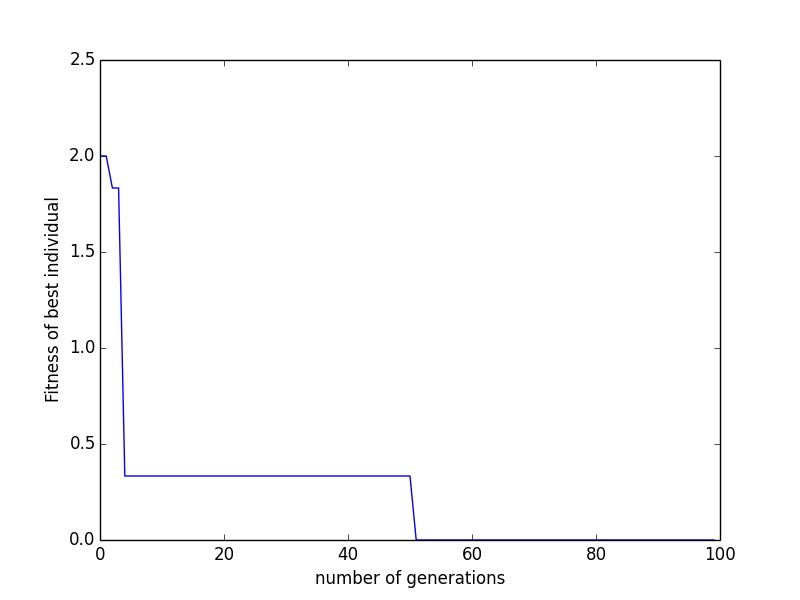
\includegraphics[scale=0.45]{./figure_BRKGA_1} 
\end{center}
\caption{ Evolution of the fitness for the TEST1.}
\label{figBRKGA_TEST1}
\end{figure}
After less than 50 generations, the fitness is 0  since all the constraints have been satisfied (Test Schedule =0) and the workload is equal to the demand. An optimal solution is then obtained. The running time is neglectible and much less than 1 second.

\vskip.5cm

\noindent
{\bf TEST2}:\\
This test optimize the schedule of 10 nurses for a 12 hours working day. After some run, we obtain a perfect scheduling using the following parameters:\\
{\tt 'chromosomeLength': 120, 'inheritanceProb': 0.7, 'numIndividuals': 100, 'eliteProp': 0.1, 'maxNumGen': 500, 'mutantProp': 0.3}\\
We obtain the optimal solution: all the schedules of the nurses satisfy the constraints, the demand is exactly satisfied. The  corresponding  fitness is represented on figure \ref{figBRKGA_TEST2} and reaches the 0 value after 60 
generations. {\tt ('Nurse', 0, 'Test Schedule =', 0)\\
('Nurse', 1, 'Test Schedule =', 0)\\
('Nurse', 2, 'Test Schedule =', 0)\\
('Nurse', 3, 'Test Schedule =', 0)\\
('Nurse', 4, 'Test Schedule =', 0)\\
('Nurse', 5, 'Test Schedule =', 0)\\
('Nurse', 6, 'Test Schedule =', 0)\\
('Nurse', 7, 'Test Schedule =', 0)\\
('Nurse', 8, 'Test Schedule =', 0)\\
('Nurse', 9, 'Test Schedule =', 0)\\
('Comp. Workload', [0, 2, 4, 5, 2, 7, 6, 4, 3, 3, 1, 1])\\
('Dema. Workload', [0, 2, 4, 5, 2, 7, 6, 4, 3, 3, 1, 1])\\
}
\vskip.5cm
\begin{figure}[htbp]
\begin{center}
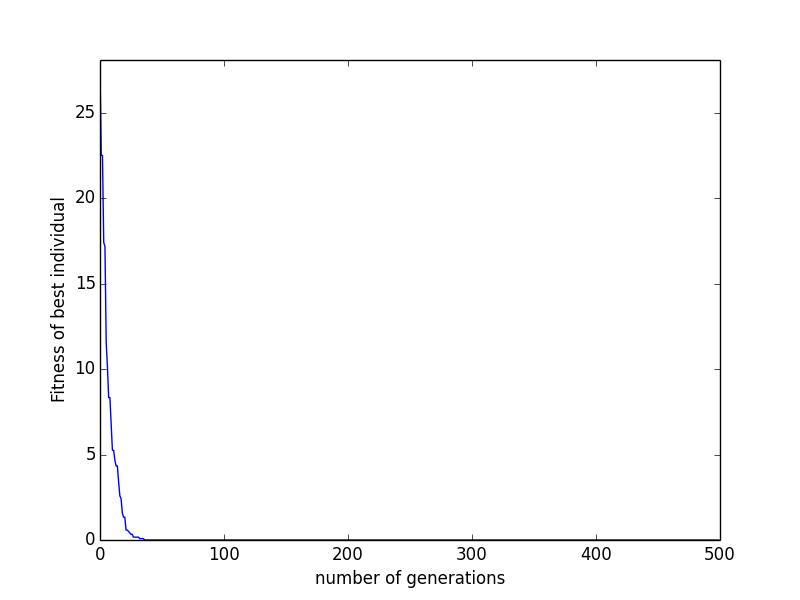
\includegraphics[scale=0.45]{./figure_BRKGA_2} 
\end{center}
\caption{ Evolution of the fitness for the TEST2.}
\label{figBRKGA_TEST2}
\end{figure}
This solution is obtain in less than 7 secondes. For all the runs we made for this TEST2, we mostly obtain a zero fitness solution in less than 1000 generations. In the case where the fitness is not 0, the schedules are always correct but the workload is overestimated since too much nurses are working comparing to the demand. This corresponds to an acceptable solution, but not the optimal one.


\vskip.5cm

\noindent
{\bf TEST3}:\\
In this test we try to optimize the schedule of 25 nurses for a 18 hours working day where the demand workload is :\\
 {\tt Dema. Workload', [9, 8, 8, 10, 11, 12, 9, 10, 16, 11, 10, 14, 13, 13, 9, 15, 12, 10]}, \\
 and  the nurses parameters:\\
 {\tt  'nNurses': 25, 'nHours': 18, 'minHours':4, 'maxHours':8, 'maxPresence':10, 'maxConsec':5}\\
 In that case, we have 450 genes for each individual of the population.\\

 One typical exemple is reported here, with the following AG parameters:\\
{\tt 'chromosomeLength': 450, 'inheritanceProb': 0.7, 'numIndividuals': 150, 'eliteProp': 0.1, 'maxNumGen': 2000, 'mutantProp': 0.3}\\
The result is not so bad since only  2 nurses have an incorrect schedule and for 2 hours the workload is not equal to the demand. The fitness evolution is reported on figure \ref{figBRKGA_TEST3A} a). As observed on figure \ref{figBRKGA_TEST3A} b), increasing the number of generations do not improve the result.\\

We perform a huge number of numerical experiments exploring  the parameters space to try to obtain the optimal solution. Unfortunately, we never obtain this optimal solution!\\
We  increase the number of mutants, and the probability of crossover, to avoid falling in a local minima but the results were not significantly better. Adding more individuals in the population do not always results in better results, but of course significantly increase the cpu time! \\

Sometimes we obtain a perfect schedule for all the 25 nurses but in that case the workload is far from the demand, and do not improves with the number of generations. We tried to find an definition of the fitness  with different amount of penalization coming from schedule and workload errors, but once again no optimal solution has been found.
\begin{figure}[htbp]
\begin{center}
\begin{tabular}{cc}
a) & b) \cr
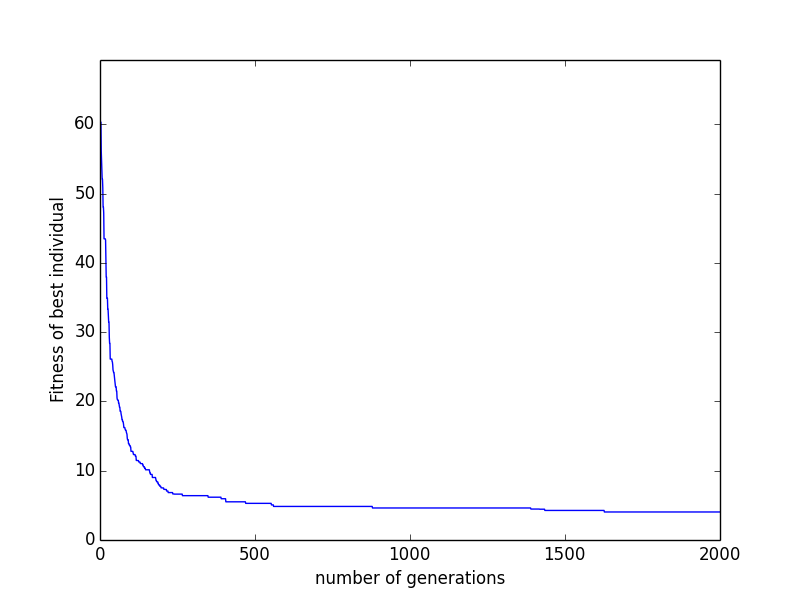
\includegraphics[scale=0.35]{./figure_BRKGA_TEST3} &
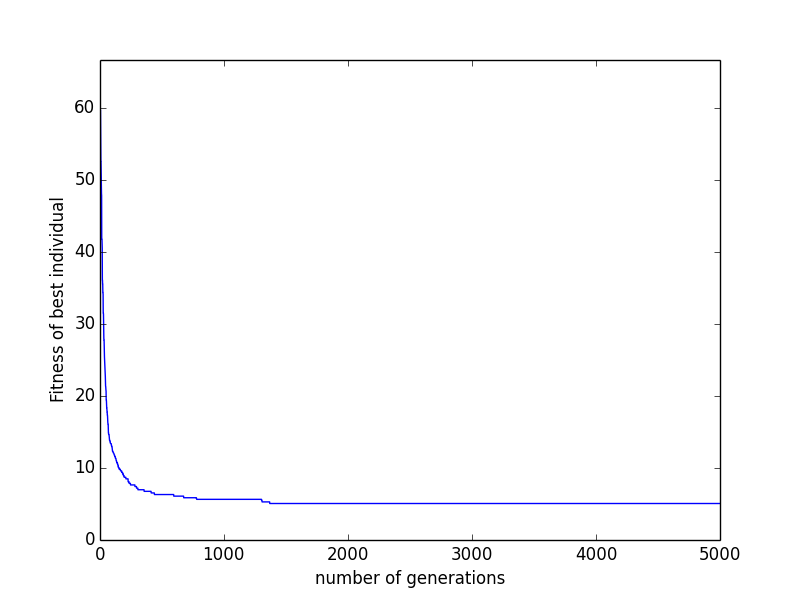
\includegraphics[scale=0.35]{./figure_BRKGA_5000} 
\end{tabular}
\end{center}
\caption{ Evolution of the fitness for the TEST3.  a) with 2000 iterations (170 sec),  b) with 5000 iterations (7 min)}
\label{figBRKGA_TEST3A}
\end{figure}


\subsection{Conclusion for BRKGA method}
We found this method very interesting since it is based on very simple concepts to optimize a complex problem. Our version gives most of the time the optimal solution for problems with less than about 350 genes. Nevertheless, we are a little bit disappointed since we do not obtain optimal results for larger problems, despite many efforts...  \\
Some improvements could be made, adding also a mutation procedure of the chromosomes, as we have seen in many AG papers. It will may be help to go out of the local minima by modifying  randomly the genes of the individuals. \\
But the best improvements would be to define a decoding procedure that gives directly a correct schedule for all the nurses. In that case, only the workload would be optimized in a very smaller space. Unfortunately, we did not found this procedure, but we will be very interesting if it exists!


%%%%%%%%%%%. GRASP section %%%%%%%

\section{The GRASP method}


%%%%%%%%%%% Apendix part.  %%%%%%%%%%%%

\pagebreak
\begin{appendix}

\section{Appendix  : OPL script }
\label{appenOPL}
\underline{OPL optimization code :}\\\\
{\tt
int numNurses = ...;\\
int hours = ...;\\
range N = 1..numNurses;\\
range H = 1..hours;\\
\\
int demand [h in H]= ...;\\
int minHours = ...;\\
int maxHours = ...;\\
int maxConsec = ...;\\
\\
int maxPresence = ...;\\
\\
dvar boolean works[n in N][h in H]; // this set of variable should suffice for A). Tells whether nurse n works at hour h\\
dvar boolean worksBefore[n in N][h in H]; // no nurse can rest more than one consec 1/3\\
dvar boolean worksAfter[n in N][h in H]; // 2/3\\
dvar boolean rests[n in N][h in H]; // 3/3\\
dvar boolean used[n in N];\\
\\\\

minimize sum(n in N) used[n]; // do not change this for A)\\
subject to $\{$\\\\
// the number of provided nurses is greater or equal to the demand\\
forall(h in H)\\
sum(n in N) works[n][h] >= demand[h]; \\
\\
// Each nurse should work at least minHours hours.\\
forall(n in N)\\
sum (h in H) works[n][h] >= minHours*used[n];\\
\\
// Each nurse should work at most maxHours hours.\\
forall(n in N)\\
sum (h in H) works[n][h] <= maxHours*used[n];\\
\\
// Each nurse should work at most maxConsec consecutive hours.\\
forall(n in N)\\
forall(i in 1..(hours-maxConsec))\\
sum(j in i..(i+maxConsec)) works[n][j] <= maxConsec*used[n];\\
\\
// No nurse can stay at the hospital for more than max Presence \\
// hours (e.g. if maxP resence is 7, it is OK that a nurse works \\
// at 2am and also at 8am, but it not possible that he/she works \\
// at 2am and also at 9am).\\
forall(n in N)\\
forall (h in H: h <= hours-maxPresence)\\
worksBefore[n][h] + worksAfter[n][h+maxPresence] <= 1;\\

forall(n in N)\\
forall (h in H: h <= hours-1)$\{$\\
worksAfter[n][h] >= worksAfter[n][h+1]; // legal: 11111110, illegal: 11111010\\
worksBefore[n][h] <= worksBefore[n][h+1]; // legal: 00011111, illegal: 00111110\\
rests[n][h] + rests[n][h+1] <= 1;\\
// legal: 00010100, illegal: 00110010\\
$\}$\\
forall(n in N)\\
forall (h in H)\\
rests[n][h] == (1-works[n][h]) - (1-worksAfter[n][h]) - (1-worksBefore[n][h]); \\
$\}$ \\
\\
execute $\{$ // Should not be changed. Assumes that variables works[n][h] are used.\\
for (var n in N) $\{$\\
write("Nurse ");\\
if (n < 10) write(" ");\\
write(n + " works: ");\\
var minHour = -1;\\
var maxHour = -1;\\
var totalHours = 0;\\
for (var h in H) $\{$\\
if (works[n][h] == 1) $\{$\\
totalHours++;\\
write(" W"); \\
if (minHour == -1) minHour = h;\\
maxHour = h; \\
$\}$\\
else write(" .");\\
$\}$\\
if (minHour != -1) write(" Presence: " + (maxHour - minHour +1));\\
else write(" Presence: 0")\\
writeln ("(TOTAL " + totalHours + "\\
$\}$\\
writeln("");\\
write("Demand: ");\\
\\
for (h in H) $\{$\\
if (demand[h] < 10) write(" ");\\
write(" " + demand[h]); \\
$\}$\\
writeln("");\\
write("Assigned: ");\\
for (h in H) $\{$\\
var total = 0;\\
for (n in N)\\
if (works[n][h] == 1) total = total+1;\\
if (total < 10) write(" ");\\
write(" " + total); \\
$\}$ \\
$\}$\\
}

%%%%%%%%%%%%%%%%%%% Appendix BRKGA %%%%%%%%%%%%%%%%%%%

\section{Appendix  : BRKGA script}
\label{appendBRKGA}
Here are the python procedures we write corresponding to the BRKGA method.\\
We apologize for the fact that  the number of hours of the day, named $hours$ in the document is called $nHours$ in the code. \\

\noindent
Transform the gene value onto a boolean value corresponding to the daily schedule\\

\noindent
{\tt def {\bf transform}(population):\\
\hspace*{.2cm}     for i in range(len(population)):\\
   \hspace*{1cm}      for j in range(len(population[i]['chr'])):\\
 \hspace*{1.5cm}            if population[i]['chr'][j] <= 1.-1.*data['minHours']/data['nHours']:\\
 \hspace*{2cm}                population[i]['solution'][j]=0\\
 \hspace*{1.5cm}            else: population[i]['solution'][j]=1\\
\hspace*{.2cm}     return population\\
 }
    
\vskip.5cm
\noindent
Check if the constraints are satisfied by the nurse schedule:\\

\noindent
{\tt def {\bf checkschedule}(currentnurse):\\
    test$=$0\\
    sumhours$=$sum(currentnurse)\\
    if sumhours $<$ data['minHours'] and sumhours $!=0$: \# Constraint minH\\
  \hspace*{1cm}       test+=1\\
    if sumhours $>$ data['maxHours']:   \#Constraint maxH\\
 \hspace*{1cm}        test+=1\\
    if sumhours $!=$ 0:        \#Constraints rests and maxPresence\\
 \hspace*{1cm}        i$=$0\\
 \hspace*{1cm}        while currentnurse[i]$==$0:\\
 \hspace*{1.5cm}            i$=$i+1\\
\hspace*{1cm}         imin$=$i\\
 \hspace*{1cm}        i=len(currentnurse)-1\\
 \hspace*{1cm}        while currentnurse[i] == 0:\\
\hspace*{1.5cm}             i = i - 1\\
\hspace*{1cm}         imax=i \\
\hspace*{1cm}         for i in range(imin, imax):\\
 \hspace*{1.5cm}            if currentnurse[i]==0 and currentnurse[i+1]==0:   \#Constraints rests\\
 \hspace*{2cm}                test+=1\\
\hspace*{1cm}         if imax-imin+1 > data['maxPresence']:       \#Constraints maxPresence\\
\hspace*{1.5cm}             test+=1\\
\hspace*{1cm}         compteur=0\\
 \hspace*{1cm}        for i in range(imin, imax+1):               \#Constraints maxConsec\\
   \hspace*{1.5cm}          if currentnurse[i]==1:\\
 \hspace*{2cm}                compteur+=1\\
 \hspace*{1.5cm}            else:\\
   \hspace*{2cm}              if compteur > data['maxConsec']:\\
\hspace*{2.5cm}                     test+=1\\
\hspace*{2cm}                 compteur = 0\\
\hspace*{1cm}         if compteur > data['maxConsec']:\\
 \hspace*{1.5cm}            test+=1\\
    return test\\
}

\vskip.5cm
\noindent
Comparison between workload and given demand:\\

\noindent
{\tt def {\bf compareworkload}(workload):\\
\hspace*{1cm}    error=0\\
\hspace*{1cm}    for i in range(0,data['nHours']):\\
\hspace*{1.5cm}        if workload[i]-data['demand'][i] > 0:\\
 \hspace*{2cm}           error+=(1.0*workload[i]-1.0*data['demand'][i])/data['nHours']\\
 \hspace*{1.5cm}       if workload[i]-data['demand'][i] < 0:\\
  \hspace*{2.cm}          error += 10.0*abs((workload[i] - data['demand'][i])) / data['nHours']\\
    return error\\
}

\vskip.5cm
\noindent
The decoder procedure:\\

\noindent
{\tt def {\bf decode}(population,data):\\
\noindent
\hspace*{1cm}   population=transform(population)\\
\noindent
\hspace*{1cm}    for x in range(len(population)):\\
\hspace*{1.5cm}        population[x]['fitness']=0\\
\hspace*{1.5cm}         workload=[0]*data['nHours']\\
\hspace*{1.5cm}         for i in range(0, data['nNurses']):\\
\hspace*{2cm}             currentnurse = []\\
\hspace*{2cm}             for j in range(i*data['nHours'], (i+1)*data['nHours']):\\
\hspace*{2.5cm}                 currentnurse.append(population[x]['solution'][j])\\
\hspace*{2cm}             test=checkschedule(currentnurse)\\
\hspace*{2cm}             \#penalize fitness if bad schedule\\
\hspace*{2cm}             population[x]['fitness'] += 10.0*test/data['nNurses']   \\
\hspace*{2cm}             for k in range(0, data['nHours']):\\
 \hspace*{2.5cm}                workload[k]+=currentnurse[k]\\
  \hspace*{1.5cm}        error=compareworkload(workload).  \\
  \hspace*{1.5cm}               \# penalize the fitness if workload error\\
 \hspace*{1.5cm}        population[x]['fitness'] +=  error. \\
    return(population)\\
}

We also define a procedure {\tt \bf infoBestIndividual} that allow us to analyze the final solution in term of schedule checking and workload demand. The script is also  in the 
DECODER$\_$DUMMY.py file.



\end{appendix}

\end{document}
